    \begin{figure}
        \centering
        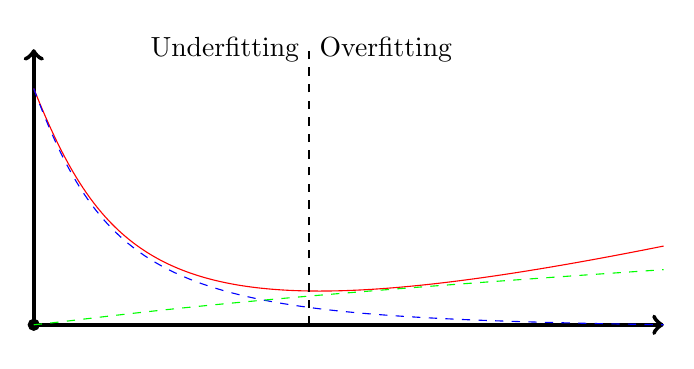
\begin{tikzpicture}
        %   \begin{axis}[ 
        %     xlabel=Capacity,
        %     xticklabels={,,},
        %     yticklabels={,,}] 
        %     % \addplot {e^(-x)}; 
        %   \end{axis}
            \draw[ultra thick, ->] (0,0.5) -- (0,4);
            \filldraw [black] (0,0.5) circle (2pt);
            \draw[ultra thick, ->] (0,0.5) -- (8,0.5);
            \draw [red] (0,3.5) .. controls (1,1) and (2,0.3) .. (8,1.5);
            \draw [blue, dashed] (0,3.5) .. controls (1,0.8) and (2,0.6) .. (8,0.5);
            \draw [green, dashed] (0,0.5) .. controls (1,0.6) and (2,0.8) .. (8,1.2);
            
            \draw[thick, dashed] (3.5, 0.5) -- (3.5, 4) node[anchor = east] {Underfitting} node[anchor = west] {Overfitting};
        \end{tikzpicture}
        \caption{Training Neural Networks can result in \textbf{underfitting} and \textbf{overfitting}; the dashed, vertical line represents the optimal training goal and divides the figure into areas of underfitting and overfitting, respectively. The Red curve is the \textit{generalization error} - which grows with the network's capacity, the blue one represents bias - which decreases with the amount of training, given enough statistical independence in the data - and the green one is the variance achieved.}
        \label{fig:over_underfitting}
    \end{figure}